\documentclass[preprint,
3p]{elsarticle} %review=doublespace preprint=single 5p=2 column
%%% Begin My package additions %%%%%%%%%%%%%%%%%%%

\usepackage[hyphens]{url}

  \journal{Atmospheric Environment} % Sets Journal name

\usepackage{graphicx}
%%%%%%%%%%%%%%%% end my additions to header

\usepackage[T1]{fontenc}
\usepackage{lmodern}
\usepackage{amssymb,amsmath}
% TODO: Currently lineno needs to be loaded after amsmath because of conflict
% https://github.com/latex-lineno/lineno/issues/5
\usepackage{lineno} % add
  \linenumbers % turns line numbering on
\usepackage{ifxetex,ifluatex}
\usepackage{fixltx2e} % provides \textsubscript
% use upquote if available, for straight quotes in verbatim environments
\IfFileExists{upquote.sty}{\usepackage{upquote}}{}
\ifnum 0\ifxetex 1\fi\ifluatex 1\fi=0 % if pdftex
  \usepackage[utf8]{inputenc}
\else % if luatex or xelatex
  \usepackage{fontspec}
  \ifxetex
    \usepackage{xltxtra,xunicode}
  \fi
  \defaultfontfeatures{Mapping=tex-text,Scale=MatchLowercase}
  \newcommand{\euro}{€}
\fi
% use microtype if available
\IfFileExists{microtype.sty}{\usepackage{microtype}}{}

\ifxetex
  \usepackage[setpagesize=false, % page size defined by xetex
              unicode=false, % unicode breaks when used with xetex
              xetex]{hyperref}
\else
  \usepackage[unicode=true]{hyperref}
\fi
\hypersetup{breaklinks=true,
            bookmarks=true,
            pdfauthor={},
            pdftitle={Reproducing the MOVES6 on-road emission-rate engine in R, row by row, for use in vehicular emission inventories of the Washington DC area},
            colorlinks=false,
            urlcolor=blue,
            linkcolor=magenta,
            pdfborder={0 0 0}}

\setcounter{secnumdepth}{5}
% Pandoc toggle for numbering sections (defaults to be off)


% tightlist command for lists without linebreak
\providecommand{\tightlist}{%
  \setlength{\itemsep}{0pt}\setlength{\parskip}{0pt}}


% Pandoc citation processing
%From Pandoc 3.1.8
% definitions for citeproc citations
\NewDocumentCommand\citeproctext{}{}
\NewDocumentCommand\citeproc{mm}{%
  \begingroup\def\citeproctext{#2}\cite{#1}\endgroup}
\makeatletter
 % allow citations to break across lines
 \let\@cite@ofmt\@firstofone
 % avoid brackets around text for \cite:
 \def\@biblabel#1{}
 \def\@cite#1#2{{#1\if@tempswa , #2\fi}}
\makeatother
\newlength{\cslhangindent}
\setlength{\cslhangindent}{1.5em}
\newlength{\csllabelwidth}
\setlength{\csllabelwidth}{3em}
\newenvironment{CSLReferences}[2] % #1 hanging-indent, #2 entry-spacing
 {\begin{list}{}{%
  \setlength{\itemindent}{0pt}
  \setlength{\leftmargin}{0pt}
  \setlength{\parsep}{0pt}
  % turn on hanging indent if param 1 is 1
  \ifodd #1
   \setlength{\leftmargin}{\cslhangindent}
   \setlength{\itemindent}{-1\cslhangindent}
  \fi
  % set entry spacing
  \setlength{\itemsep}{#2\baselineskip}}}
 {\end{list}}
\usepackage{calc}
\newcommand{\CSLBlock}[1]{#1\hfill\break}
\newcommand{\CSLLeftMargin}[1]{\parbox[t]{\csllabelwidth}{#1}}
\newcommand{\CSLRightInline}[1]{\parbox[t]{\linewidth - \csllabelwidth}{#1}\break}
\newcommand{\CSLIndent}[1]{\hspace{\cslhangindent}#1}


\usepackage{booktabs}
\usepackage{amsmath}
\usepackage{array}



\begin{document}


\begin{frontmatter}

  \title{Reproducing the MOVES6 on-road emission-rate engine in R, row
by row, for use in vehicular emission inventories of the Washington DC
area}
    \author[a]{Sergio Ibarra-Espinosa%
  \corref{cor1}%
  }
   \ead{zergioibarra@gmail.com} 
      \affiliation[a]{
    organization={Cooperative Institute for Satellite Earth System
Studies (CISESS) and Earth System Science Interdisciplinary Center
(ESSIC), University of Maryland},city={College
Park},state={MD},country={USA},}
    \cortext[cor1]{Corresponding author}
  
  \begin{abstract}
  The U.S. EPA Motor Vehicle Emission Simulator (MOVES) is the
  regulatory model for on-road emissions in the United States, but
  running it requires a Java application, a MariaDB server, compiled Go
  programs and a full database installation. This makes MOVES hard to
  embed in inventory models such as VEIN. We describe movesr, an R
  package that reimplements the MOVES6.0.0 rate engine using the MOVES
  default database stored as Parquet files. The port covers running and
  start exhaust, brake and tire wear, evaporative permeation, vapor
  venting and fuel leaks (parked and while driving), and the chained
  pollutants (CH4, NMHC, NMOG, TOG, VOC, CO2, CO2e, SO2, PM2.5 species
  and PM10). Each MOVES step was translated from the Java, SQL and Go
  source code and checked against MOVES execution tables and final
  outputs. We compared 4,302,126 MOVES6 rates from five reference runs
  (Washtenaw County MI and the District of Columbia, Montgomery County
  MD and Fairfax County VA). Every rate was reproduced. For exhaust,
  brake and tire rates the largest relative difference was
  \(1.6 \times 10^{-5}\), which is at the level of the six significant
  digits that MOVES writes. Evaporative rates agreed within
  \(2.9 \times 10^{-5}\) at the 99th percentile; the largest difference,
  \(8.7 \times 10^{-4}\), occurred in E85 vapor venting, which amplifies
  single-precision rounding of tank temperatures. We also describe a
  simplified evaporative method that replaces the MOVES trip simulation
  by interpolation in a library of exact results. It reproduces
  permeation and leak daily totals within 0.44\% and vapor venting
  within 3.8\% on average, but saves little time in a single run. On the
  same workstation, movesr produced the rates of each reference run 3.7
  to 9.2 times faster than MOVES with one worker, using about three
  times more memory than the largest MOVES process. Factors written by
  movesr are read by VEIN without loss. The paper documents the
  procedure that makes the numbers identical across MOVES, movesr and
  VEIN, and the MOVES behaviours that a reimplementation must reproduce.
  \end{abstract}
    \begin{keyword}
    MOVES \sep Emission factors \sep Vehicular emissions
inventory \sep Evaporative emissions \sep Reproducibility \sep 
    R
  \end{keyword}
  
 \end{frontmatter}

\section{Introduction}\label{introduction}

Bottom-up vehicular emission inventories combine traffic activity with
emission factors. In the United States the regulatory source of on-road
emission factors is the Motor Vehicle Emission Simulator, MOVES (U.S.
Environmental Protection Agency, 2026a, 2026b). MOVES combines a large
default database (fleet, activity, fuels, meteorology, inspection and
maintenance programs) with emission rates by operating mode, and
produces either inventories or rate tables. EPA guidance allows MOVES to
be run in ``rates'' mode so that its output, in grams per mile, per
start or per vehicle, can be multiplied by activity in an external model
(U.S. Environmental Protection Agency, 2026b).

VEIN is an R package for vehicular emission inventories
(Ibarra-Espinosa, 2026a; Ibarra-Espinosa et al., 2018). It already reads
MOVES rate tables, but producing those tables still requires MOVES
itself. MOVES6 is a Java application that stores every intermediate
table in MariaDB, delegates parts of the computation to programs written
in Go, and needs the complete default database to be installed. A single
run for three counties, two hours and all source types took close to an
hour on our workstation with one worker (Section \ref{sec:time}). For an
inventory with many counties, months and hours this is a practical
limit, and the dependency stack makes it hard to run MOVES inside other
modelling systems or to inspect intermediate results.

This paper describes movesr (Ibarra-Espinosa, 2026b), an R package that
reproduces the MOVES6.0.0 rate engine without Java, MariaDB or MOVES.
The objective is narrow: for the same inputs, movesr must return the
same numbers as MOVES, rate by rate, so that an inventory built with
VEIN gives the same result whether the factors came from MOVES or from
movesr. We do not propose new emission science. We document how each
MOVES step was reproduced, how equality was verified, which MOVES
behaviours a faithful port must keep, and where movesr departs from
MOVES on purpose (a simplified evaporative method). The work prepares a
VEIN inventory for the Washington DC area, so the reference runs use the
District of Columbia and two neighbouring counties.

The code was written with the help of a large language model working as
a coding agent. Section \ref{sec:ai} describes how, and which model. We
report this because it matters for how much trust readers should place
in the software: the evidence of correctness in this paper comes from
comparison with MOVES outputs, not from the way the code was written.

\section{Methods}\label{methods}

\subsection{\texorpdfstring{Reference model and reference runs
\label{sec:runs}}{Reference model and reference runs }}\label{reference-model-and-reference-runs}

The reference is MOVES6.0.0 (U.S. Environmental Protection Agency,
2026c), source commit \texttt{45805553} (full hash in the reference
list), with the default database \texttt{movesdb20260729}. MOVES was
compiled and run on Linux with Java 11.0.10, Go 1.26.10 and MariaDB
10.11.14, using a private database server and a single worker, so that
runs were deterministic and isolated from other work. Five reference
runs (``golden sets'') were made with the real model (Table
\ref{tab:golden}). The RunSpecs are stored in the movesr repository
(\texttt{data-raw/dmv/*.mrs}) and in VEIN
(\texttt{inst/extdata/moves/*.mrs}), together with the script that
starts the database, runs MOVES, exports the output tables and shuts the
server down (\texttt{data-raw/dmv/generate\_dmv.py}). Besides the final
rate tables, the script exports MOVES execution tables (activity, tank
temperatures, soak fractions, coefficients) so that intermediate steps
can be checked one at a time.

\begin{table}

\caption{\label{tab:golden}MOVES6 reference runs. All runs use all 13 source types and every valid fuel, model years 1985 to 2025 (Washtenaw: 2000 to 2025), urban unrestricted roads for distance rates, and MOVES defaults for fleet, fuels and inspection programs.}
\centering
\small\begin{tabular}[t]{>{\raggedright\arraybackslash}p{2.2cm}>{\raggedright\arraybackslash}p{3.6cm}>{\raggedright\arraybackslash}p{4cm}>{\raggedright\arraybackslash}p{4.6cm}}
\toprule
Run & Location & Time & Processes\\
\midrule
Washtenaw running & Washtenaw County MI (26161) & 2025, January, weekend day, hours 1 to 3 (20, 10 and 30 C, 50\% RH; 20 C in other hours) & Running (1): CO, NOx\\
Washtenaw events & Washtenaw County MI (26161) & Same as Washtenaw running & Start (2): CO, NOx; evaporative (11 to 13) off network: THC\\
DMV running & DC (11001), Montgomery MD (24031), Fairfax VA (51059) & 2025, July, weekday, hours 16 and 17, default weather & Running (1), brake (9), tire (10), evaporative (11 to 13) on roads; 21 pollutants\\
DMV events & Same three counties & 2025, July, weekday, hours 16 and 17, default weather & Start (2), evaporative (11 to 13) off network\\
DC 24 h evaporative & District of Columbia (11001) & 2025, July, weekday, hours 1 to 24, default weather & Evaporative (11 to 13); THC, NMHC, NMOG, TOG, VOC\\
\bottomrule
\end{tabular}
\end{table}

The two Washtenaw runs are the reference data distributed with VEIN. The
three DMV counties belong to the Washington DC-MD-VA ozone nonattainment
area (U.S. Environmental Protection Agency, 2026d); movesr includes the
15 jurisdictions of that area as a predefined region.

\subsection{Porting rules}\label{porting-rules}

The port follows four rules.

\begin{enumerate}
\def\labelenumi{\arabic{enumi}.}
\tightlist
\item
  \emph{Read the code that actually runs.} MOVES6 contains several
  implementations of the same step. For example, drive-cycle operating
  modes are computed by a Go program
  (\texttt{generators/baserategenerator}) because a compilation flag
  (\texttt{USE\_EXTERNAL\_GENERATOR\_FOR\_DRIVE\_CYCLES}) is set; the
  Java SQL in \texttt{RatesOperatingModeDistributionGenerator} is not
  used and gives different results for heavy-duty cycles. Vapor venting
  uses \texttt{MultidayTankVaporVentingCalculator.sql} because
  \texttt{USE\_MULTIDAY\_DIURNALS} is true, not the older
  \texttt{TankVaporVentingCalculator.sql}. Each movesr function names
  the MOVES file it reproduces.
\item
  \emph{Check every stage against MOVES.} When MOVES writes an
  intermediate table to its execution database, the corresponding movesr
  table was compared with it before the next stage was written.
\item
  \emph{Compare all rows.} Every rate of every reference run is
  compared, matched on all key columns (county or zone, hour, source
  type, fuel type, model year, pollutant, process, road type, speed
  bin). A rate present in MOVES and absent in movesr, or the reverse, is
  reported as a failure, not dropped.
\item
  \emph{Keep MOVES arithmetic.} MOVES stores most intermediate values in
  single-precision \texttt{FLOAT} columns and the tank temperature
  generator uses Java \texttt{float}. Where this changes results beyond
  the output precision, movesr rounds to single precision at the same
  points (\emph{{IEEE} standard for floating-point arithmetic}, 2019).
  Elsewhere it uses double precision.
\end{enumerate}

movesr is written in R (R Core Team, 2021) with data.table (Barrett et
al., 2026). It runs in one thread and has no compiled code. Figure
\ref{fig:structure} shows how the MOVES stages map to movesr functions
and where the comparison with MOVES enters.

\begin{figure}[htbp]

{\centering 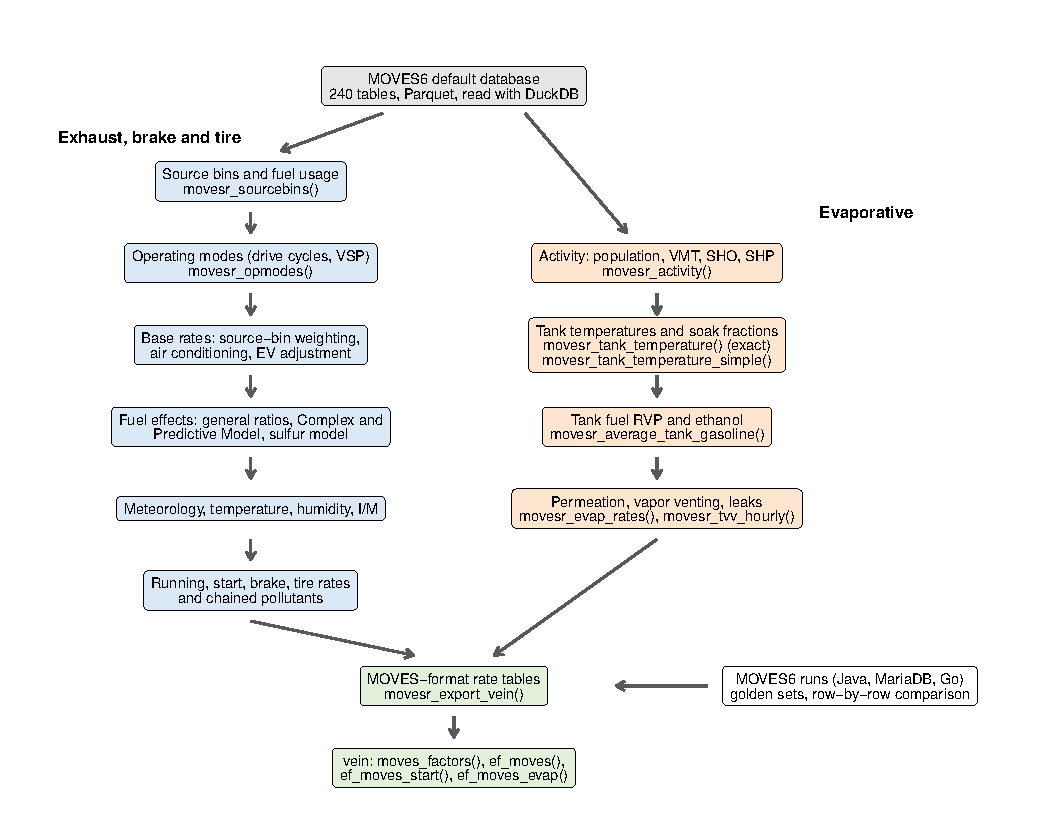
\includegraphics[width=0.85\linewidth]{figures/fig1_structure} 

}

\caption{Structure of movesr. Each box is a MOVES stage and the movesr function that reproduces it; the reference runs of MOVES6 are compared with the rate tables that movesr writes. \label{fig:structure}}\label{fig:fig-structure}
\end{figure}

\subsection{Default database}\label{default-database}

The MOVES default database (240 tables) was converted once to Apache
Parquet (The Apache Software Foundation, 2026) with DuckDB (Raasveldt
and Mühleisen, 2019) through its MySQL extension. Row counts of all
tables were compared with the MariaDB source (no differences), and a
SHA-256 hash of each file is stored in a catalog. The Parquet files
total 10 MiB. movesr reads them through the DuckDB command-line program,
so it needs neither a database server nor the \texttt{arrow} R package.
Tables that MOVES fills during a run (source-bin distributions,
operating-mode distributions, fuel adjustments, activity) are empty in
the default database; movesr computes them.

\subsection{Running exhaust (process
1)}\label{running-exhaust-process-1}

\emph{Source bins.} A MOVES source bin combines fuel, engine technology,
regulatory class and model-year group. Its activity share within a
source type and model year is the sum of \texttt{stmyFraction} in
\texttt{SampleVehiclePopulation}. Regulatory class and model-year group
enter the bin only when \texttt{SourceTypePolProcess} requires them
(\texttt{isRegClassReqd}, \texttt{isMYGroupReqd}).
\texttt{FuelUsageFraction} then moves activity from the equipped fuel to
the fuel actually used, so that, for example, most flex-fuel activity is
reported as gasoline.

\emph{Operating modes.} For each source type, road type and
average-speed bin, MOVES brackets the bin speed between two drive
schedules and weights them by distance in speed. For each second of a
schedule the Go generator computes the vehicle specific power
(Jiménez-Palacios, 1999) from the road-load coefficients of
\texttt{SourceUseTypePhysics}: \begin{equation}
\mathrm{VSP} = \frac{A v + B v^2 + C v^3 + M v a}{f_m},
\end{equation} with \(v\) and \(a\) in m s\(^{-1}\) and m s\(^{-2}\) and
\(f_m\) the fixed mass factor. Speed below 1 mph is idle (mode 1);
braking (mode 0) is \(a \le -2\) mph s\(^{-1}\), or three consecutive
seconds below \(-1\) mph s\(^{-1}\). The Go code sets the acceleration
to zero when the previous second is missing, which happens in heavy-duty
schedules; the first port computed accelerations across those gaps and
failed the comparison until this was reproduced. Speed bounds of the
operating modes are in mph. One distribution is produced per row of
\texttt{SourceUseTypePhysics} (source type, regulatory class, model-year
range).

\emph{Base rates.} Rates are averaged over source bins with their
activity shares, separately for the mean rate, the I/M rate and the
air-conditioning increment: \begin{equation}
\mathrm{MBR} = \frac{\sum_b s_b\,r_b}{\sum_b s_b}, \qquad
\mathrm{ER} = \frac{\sum_m \mathrm{MBR}_m\,f_m}{\bar{v}} \;\; [\mathrm{g\,mile^{-1}}],
\end{equation} where \(s_b\) is the source-bin share, \(r_b\) the
\texttt{EmissionRateByAge} value, \(f_m\) the operating-mode fraction
and \(\bar v\) the bin speed. An electric-vehicle adjustment raises
non-electric rates when the fleet-average standard is met partly by
electric sales.

\emph{Corrections.} The calculator applies, per fuel formulation, the
fuel-effect ratio, a temperature factor \(1 + (t-75)(A + (t-75)B)\), the
NOx humidity factor \(K = 1 - 0.0329\,(H - 10.71)\) with \(H\) in g
kg\(^{-1}\) bounded to \([3, 17.71]\), the air-conditioning factor from
the heat index, and the I/M fraction
\(f = \sum \mathrm{IMFactor}\times\mathrm{compliance}/100\):
\begin{equation}
r = R \cdot T \cdot \left[(1-f)(\mathrm{ER} + \mathrm{AC}\,\mathrm{ER}_{AC}) + f(\mathrm{ER}_{IM} + \mathrm{AC}\,\mathrm{ER}_{IM,AC})\right].
\end{equation} Fuel-effect ratios come from
\texttt{GeneralFuelRatioExpression}, which stores MySQL expressions;
movesr translates them to R and evaluates them for each formulation of
the fuel supply. High-ethanol fuels take E10 properties as MOVES does.
Model years without an expression use the Complex Model (CO) or the
Predictive Model (THC, NOx) followed by the sulfur model. The result is
weighted by market share and by the gasoline program area fraction.

\emph{Regulatory classes.} Rates computed by regulatory class are
combined with weights equal to the source-bin activity shares, which is
what the Go code does in \texttt{calculateActivityWeight}. Ages with no
population give a zero rate, as in MOVES.

\subsection{Start exhaust (process 2)}\label{start-exhaust-process-2}

Start rates use operating modes 101 to 108 (soak-time classes) from
\texttt{StartsOpModeDistribution}, by source type, hour and day type.
Each mode rate receives the start temperature adjustment (polynomial or
logarithmic by fuel, pollutant and model-year group, using
\(\min(t, 75) - 75\)), then the same fuel, temperature, I/M,
electric-vehicle and regulatory-class stages as running rates, without
air conditioning.

\subsection{Brake and tire wear (processes 9 and
10)}\label{brake-and-tire-wear-processes-9-and-10}

Brake-wear operating modes come from the same Go drive-cycle generator
as running exhaust, and tire-wear modes from the speed classes of
\texttt{AverageSpeedOperatingModeDistributionGenerator}. Their bins
carry model-year group 0, so \texttt{SourceTypePolProcess} decides the
bin structure. PM10 comes from PM2.5 through \texttt{PM10PM25Ratio}.

\subsection{Chained pollutants}\label{chained-pollutants}

Chained pollutants are computed per regulatory class, before
aggregation. CH4 and NMHC follow from THC and \texttt{MethaneTHCRatio};
NMOG and VOC from NMHC and \texttt{HCSpeciation}, using the oxygenate
content of each formulation; TOG is NMOG plus CH4. For E85 vehicles from
model year 2001, NMOG and VOC use an alternative THC evaluated with E10
RVP, as in the Go calculator. CO2 follows from energy, carbon content
and oxidation fraction, CO2e from CO2, CH4 and N2O with global warming
potentials, and SO2 from energy and fuel sulfur. PM2.5 is split into
elemental carbon, sulfate, aerosol water and the remainder, with the
sulfur adjustment and the crankcase split of
\texttt{SulfatePMCalculator.sql}.

\subsection{Evaporative emissions (processes 11, 12,
13)}\label{evaporative-emissions-processes-11-12-13}

Evaporative emissions needed four parts of MOVES that the exhaust
processes do not use.

\emph{Activity.} From \texttt{TotalActivityGenerator} and
\texttt{ActivityCalculator.sql}, movesr computes population by source
type and age, travel fractions within each HPMS vehicle class, annual
and hourly VMT, source hours operating (SHO = VMT / average speed) and
source hours parked: \begin{equation}
\mathrm{SHP} = P \cdot N_d - \sum_{\mathrm{roads}} \mathrm{SHO},
\end{equation} where \(P\) is population and \(N_d\) the number of real
days in the day type (5 for weekdays). The zone population is \(P\)
times the zone's share of source hours operating
(\texttt{SHOAllocFactor}), averaged over road types with their VMT
fractions. MOVES reports evaporative rates as emissions divided by
population, so the per-vehicle rate equals the rate per parked hour
times \(\mathrm{SHP}\cdot\alpha/(P_z N_d)\), with \(\alpha\) the zone
allocation factor.

\emph{Tank temperatures.} \texttt{TankTemperatureGenerator} simulates
the sample vehicles of the day type (about 11,000 vehicles and 27,000
trips for weekdays). The cold-soak tank temperature follows the ambient
profile with a quarter-hour recursion. During a trip the tank warms as
\begin{equation}
T_{off} = T_{on} + \frac{A + B\,(95 - T_{on})}{1.2}\,\frac{\Delta t}{60}, \qquad T_{off} \le 140\ \mathrm{F},
\end{equation} with \(A\) and \(B\) by tank temperature group (for
passenger cars from model year 1996, \(A = 24\) and \(B = -0.352\)).
After the trip the tank cools minute by minute,
\(T = T_{off} + 1.4 \sum (T_{amb} - T)/60\), until it is within 3 F of
the cold-soak temperature; the next trip starts from the soak
temperature. From this simulation MOVES derives the average tank
temperature of each hour for hot soak (mode 150), cold soak (151) and
operating (300), the share of parked time in hot and cold soak, and the
cold-soak initial-hour fractions (the hour at which each cold-soaking
vehicle began to soak). MOVES uses Java \texttt{float} in this code, and
movesr emulates it.

\emph{Tank fuel.} \texttt{TankFuelGenerator} computes the tank RVP from
the market-share average fuel with the Reddy blending relation,
weathered with an evaporation temperature derived from the monthly
minimum and maximum temperatures, and corrected for commingling of
ethanol and non-ethanol fuels.

\emph{Calculators.} With \(f_m\) the operating-mode fractions (hot and
cold soak from the soak shares, operating the remainder): \begin{align}
\text{permeation} &= \mathrm{MBR}\cdot F_{EtOH} \sum_m A\,e^{B\,T_{tank,m}} f_m, \\
\text{leaks} &= \sum_m \mathrm{MBR}_m f_m, \\
\text{venting} &= \sum_{bins} s_b\,\mathrm{TVV}_{h} f_{151} + \mathrm{MBR}_{150} f_{150} + \mathrm{MBR}_{300}\,\tau(t)\,\rho(t, \mathrm{RVP})\,f_{300},
\end{align} followed by the I/M combination. \(F_{EtOH}\) is the
permeation fuel adjustment by ethanol level, and \(\tau\) and \(\rho\)
are the temperature and RVP adjustments of
\texttt{EvapTemperatureAdjustment} and
\texttt{EvapRVPTemperatureAdjustment}. The hourly cold-soak vented vapor
\(\mathrm{TVV}_h\) is the most involved part of MOVES. For each pair of
initial hour \(I\) and current hour \(h\) up to the hour of peak tank
temperature, the tank vapor generated is \begin{equation}
\mathrm{TVG}(I,h) = V_{tank}(1 - \phi)\,a\,e^{b\,\mathrm{RVP}}\left(e^{c T_h} - e^{c T_I}\right),
\end{equation} interpolated between low- and high-altitude coefficients
by barometric pressure and between E0 and E10 by tank ethanol. The
canister load over five soak days is \begin{equation}
X_1 = \mathrm{TVG}_{I..h}, \quad X_2 = (1-\beta)\min(\mathrm{TVG}_{I..24}, C) + \mathrm{TVG}_{1..h}, \quad X_n = (1-\beta)\min(X_{n-1} + \mathrm{TVG}_{h+1..24}, C) + \mathrm{TVG}_{1..h},
\end{equation} with back-purge factor \(\beta\) and canister capacity
\(C\). The vented vapor is the regulatory-class weighted combination of
the \texttt{cumTVVCoeffs} vent and leak equations, which are stored as
SQL text; movesr evaluates them in R. Hourly increments are kept only
while the tank temperature rises, weighted by the initial-hour fractions
(day 1) and by the multiday soaking fractions (days 2 to 5), and the
four hours after the peak receive 2, 1, 0.4 and 0.05\% of the peak-hour
value.

All evaporative rates are computed by regulatory class (MOVES always
enables its \texttt{WithRegClassID} sections), speciated, and then
summed. Permeation bins carry no regulatory class, so they are split
with \texttt{RegClassSourceTypeFraction}, which movesr rebuilds from
\texttt{UpdateExecution.sql}. On roads only mode 300 applies and the
rate per distance is the operating rate divided by the bin speed.

\subsection{\texorpdfstring{Simplified evaporative method
\label{sec:simple}}{Simplified evaporative method }}\label{simplified-evaporative-method}

The trip simulation is the slowest step of the evaporative chain. The
simplified method keeps everything else and replaces only the
simulation. The cold-soak tank temperature is still computed exactly.
The rise of hot-soak and operating tank temperatures over the cold-soak
temperature, the soak shares and the initial-hour fractions are
interpolated from a library of exact results. The library holds 113
MOVES default 24-hour temperature profiles per day type, chosen to cover
U.S. climates (20 bins of daily mean temperature, 5 bins of diurnal
range, and 13 profiles in the tails). For a new profile the three
library profiles nearest in daily mean and diurnal range are combined
with inverse squared distance weights, and a warning is issued when the
nearest is more than 5 F away. Matching hour by hour on ambient and
cold-soak temperature was tested and was not more accurate.

\subsection{Comparison statistic and the precision
bound}\label{comparison-statistic-and-the-precision-bound}

For each matched pair of rates we compute the relative difference
\(\delta = r_{\mathrm{movesr}}/r_{\mathrm{MOVES}} - 1\), with
\(\delta = 0\) when both are zero. A pair where MOVES is zero and movesr
is not, or the reverse, would give an infinite \(\delta\) and is counted
as a failure; none occurred. MOVES writes its output tables from
single-precision columns, which MariaDB prints with six significant
digits. Rounding a positive number to six significant digits changes it
by at most \(5\times10^{-6}\) in relative terms, and single-precision
storage adds about \(6\times10^{-8}\) per operation. Differences up to
about \(10^{-5}\) therefore carry no information about the method. We
report the median, the 99th percentile and the maximum of \(|\delta|\),
and the number of rates above \(10^{-5}\) and \(10^{-4}\).

\subsection{Replication protocol}\label{replication-protocol}

The steps needed to obtain the same numbers with MOVES, movesr and VEIN
are:

\begin{enumerate}
\def\labelenumi{\arabic{enumi}.}
\tightlist
\item
  Use MOVES6.0.0 at commit \texttt{45805553} with the default database
  \texttt{movesdb20260729}, and the RunSpecs in the repositories. Any
  other MOVES version or database changes the reference.
\item
  Convert the default database to Parquet once and check the stored
  SHA-256 hashes.
\item
  Give movesr the same location (county), calendar year, month, day
  type, hours, hourly temperature and relative humidity, and the same
  road types and source types as the RunSpec. Evaporative rates need the
  24 hours of the day, because tank temperatures depend on the whole
  diurnal cycle.
\item
  Run \texttt{paper/scripts/01\_parity.R}, which recomputes all
  comparisons from the MOVES exports, then \texttt{02\_simplified.R},
  \texttt{03\_vein\_roundtrip.R}, \texttt{05\_venting\_hours.R},
  \texttt{06\_timing.sh} (which repeats the MOVES runs),
  \texttt{07\_moves\_repeat.R} and \texttt{04\_figures.R}. All numbers
  in this paper are read from the files these scripts write.
\item
  To use the factors in VEIN, export them with
  \texttt{movesr\_export\_vein()} and read them with
  \texttt{moves\_factors()}, \texttt{moves\_start\_factors()} and
  \texttt{moves\_evap\_factors()}. These functions keep MOVES units and
  convert g/mile to g/km only by dividing by 1.609344.
\end{enumerate}

The movesr test suite contains the same checks on a subset of the golden
sets and runs them when the MOVES exports are available.

\section{Results}\label{results}

\subsection{Agreement with MOVES}\label{agreement-with-moves}

\begin{table}

\caption{\label{tab:parity-table}Relative difference $|\delta|$ between movesr and MOVES6 for every rate of the reference runs. Missing: rates written by MOVES and not produced by movesr. \label{tab:parity}}
\centering
\begin{tabular}[t]{llrrrrrrr}
\toprule
Run & Rates & Compared & Missing & Median & 99th pct. & Max. & > 1e-5 & > 1e-4\\
\midrule
Washtenaw & running & 86,304 & 0 & $7 \times 10^{-7}$ & $4.2 \times 10^{-6}$ & $6.5 \times 10^{-6}$ & 0 & 0\\
Washtenaw & start & 5,394 & 0 & $6.2 \times 10^{-7}$ & $4.7 \times 10^{-6}$ & $7.2 \times 10^{-6}$ & 0 & 0\\
Washtenaw & evap parked & 3,186 & 0 & $2.3 \times 10^{-6}$ & $1.6 \times 10^{-5}$ & $2.9 \times 10^{-5}$ & 104 & 0\\
DMV & running & 2,522,784 & 0 & $7 \times 10^{-7}$ & $4.2 \times 10^{-6}$ & $1.6 \times 10^{-5}$ & 156 & 0\\
DMV & brake/tire & 529,536 & 0 & $6.7 \times 10^{-7}$ & $4.1 \times 10^{-6}$ & $7.8 \times 10^{-6}$ & 0 & 0\\
DMV & start & 155,112 & 0 & $5.7 \times 10^{-7}$ & $4.2 \times 10^{-6}$ & $6.6 \times 10^{-6}$ & 0 & 0\\
DMV & evap parked & 47,610 & 0 & $2.3 \times 10^{-6}$ & $1.1 \times 10^{-5}$ & $2.1 \times 10^{-5}$ & 806 & 0\\
DMV & evap driving & 761,760 & 0 & $2.4 \times 10^{-6}$ & $2 \times 10^{-5}$ & $3.5 \times 10^{-5}$ & 78,062 & 0\\
DC 24 h & evap parked & 190,440 & 0 & $2.4 \times 10^{-6}$ & $2.9 \times 10^{-5}$ & $8.7 \times 10^{-4}$ & 7,232 & 353\\
\bottomrule
\end{tabular}
\end{table}

Table \ref{tab:parity} and Figures \ref{fig:parity} and
\ref{fig:reldiff} summarise the comparison (the Washtenaw evaporative
rates are in the table but not in the figures). movesr reproduced all
4,302,126 rates, with no missing or extra rates. For running and start
exhaust, brake and tire wear, the largest difference was
\(1.6 \times 10^{-5}\) and almost all differences fall in the decades
\(10^{-8}\) to \(10^{-6}\), the range expected from MOVES output
rounding. The few exhaust rates between \(10^{-5}\) and
\(2\times10^{-5}\) are energy consumption (pollutant 91), which MOVES
reports in joules with large magnitudes and therefore more
single-precision rounding before printing.

Evaporative rates agree within \(2.9 \times 10^{-5}\) at the 99th
percentile. The largest differences are in vapor venting of E85 vehicles
during the hours of rising temperature. Venting is computed from hourly
differences of cumulative single-precision values and from exponentials
of tank temperatures, so a change of \(10^{-5}\) F in a tank temperature
is amplified. MOVES writes tank temperatures with four decimals, which
is not enough to remove this sensitivity: when movesr was fed the
cold-soak temperatures as printed by MOVES, instead of computing them,
the maximum difference grew to \(2.7\times10^{-3}\). We therefore
attribute the residual to single-precision rounding inside MOVES rather
than to a different method, although we could not verify this directly
because the unrounded MOVES values are not available. On roads, 77,207
of the 253,920 permeation rates differ by more than \(10^{-5}\) (maximum
\(3.5 \times 10^{-5}\)). Permeation depends exponentially on the
operating tank temperature, which movesr computes in the same
single-precision steps as MOVES but cannot match bit for bit.

The Washtenaw evaporative rates are for a weekend day in January and
were the only weekend evaporative rates available. All 3,186 of them
were reproduced within \(2.9 \times 10^{-5}\), but only after one
setting was changed. With the E85 tank fuel built from the E85
formulation as supplied (the setting that reproduced the DMV events and
DC 24-hour runs), 63 E85 venting rates at hour 3 were 1.7\% too low.
With the E85 formulation carrying E10 properties, as
\texttt{FuelEffectsGenerator} leaves it, they matched. The same E10
setting was needed for the DMV running run (Section \ref{sec:quirks}).
movesr also returns rates for model years 1985 to 1999, which this
reference run does not contain.

MOVES itself is not exactly repeatable at this level. Running the three
DMV and DC RunSpecs a second time (for the timing in Section
\ref{sec:time}) gave the same 4,361,724 non-null rates, of which 15,022
differed from the first run, by up to \(1 \times 10^{-5}\). Differences
of this size between movesr and MOVES are therefore within the
run-to-run variation of MOVES.

\begin{figure}[htbp]
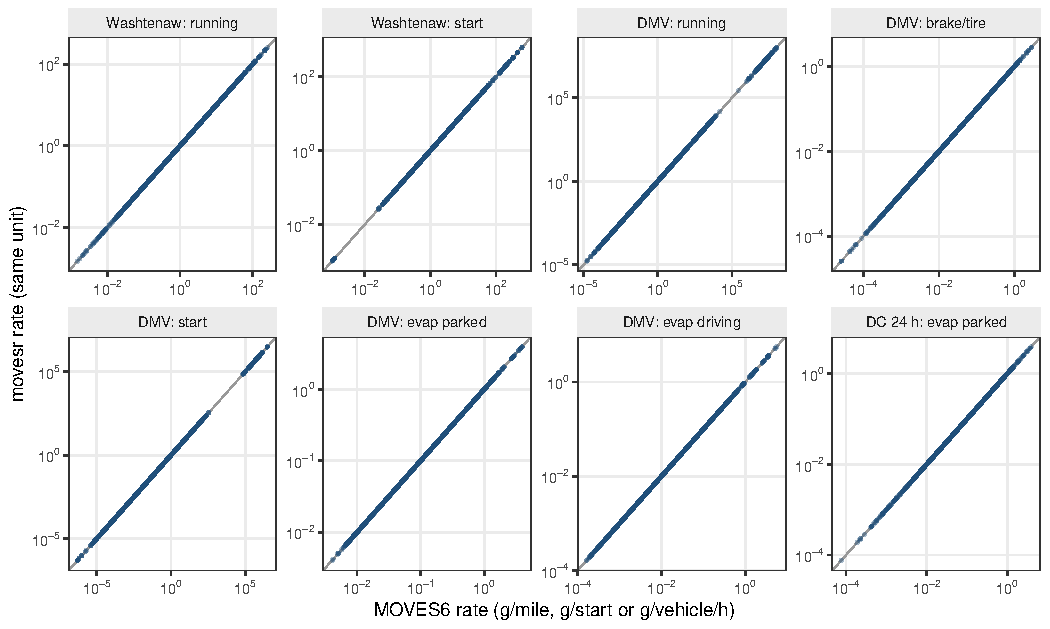
\includegraphics[width=1\linewidth]{figures/fig2_parity} \caption{movesr rates against MOVES6 rates for every reference run (random sample of up to 4,000 rates per panel; all rates are compared in Table \ref{tab:parity}). \label{fig:parity}}\label{fig:fig-parity}
\end{figure}

\begin{figure}[htbp]
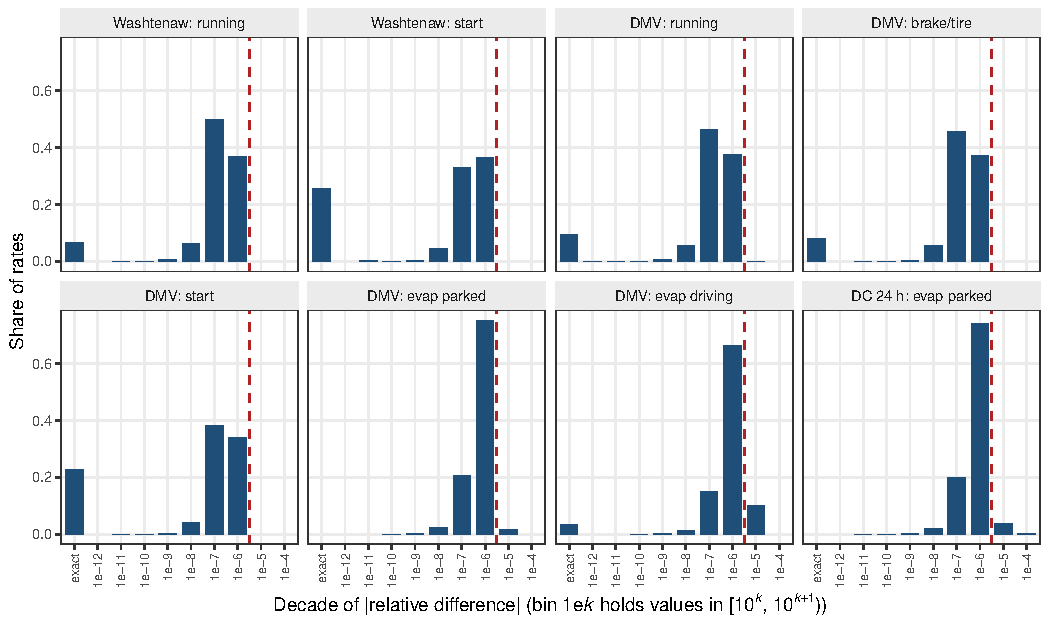
\includegraphics[width=1\linewidth]{figures/fig3_reldiff} \caption{Distribution of the relative difference between movesr and MOVES6 by decade, for all rates. The dashed line marks $10^{-5}$; MOVES output rounding alone gives differences up to $5 \times 10^{-6}$. \label{fig:reldiff}}\label{fig:fig-reldiff}
\end{figure}

\subsection{Intermediate tables}\label{intermediate-tables}

Table \ref{tab:inter} compares intermediate evaporative tables for the
District of Columbia with the MOVES execution database. Population, SHO
and SHP agree to the precision of the exported values. Average tank
temperatures agree within \(5\times10^{-4}\) F, which is the last
printed digit, soak shares within \(5\times10^{-7}\), and initial-hour
fractions within \(5\times10^{-6}\). Figure \ref{fig:tank} shows the
tank temperatures of passenger cars over the day.

\begin{table}

\caption{\label{tab:inter-table}movesr against MOVES execution tables, District of Columbia, July weekday. Every row exported by MOVES was matched; MOVES exported soak activity fractions only for hours 16 and 17. \label{tab:inter}}
\centering
\begin{tabular}[t]{llll}
\toprule
Table & Rows compared & Max. difference & Unit\\
\midrule
AverageTankTemperature, mode 150 & 384 & $5 \times 10^{-4}$ & F\\
AverageTankTemperature, mode 151 & 384 & $4.9 \times 10^{-5}$ & F\\
AverageTankTemperature, mode 300 & 384 & $5 \times 10^{-4}$ & F\\
ColdSoakTankTemperature & 24 & $4.9 \times 10^{-5}$ & F\\
SoakActivityFraction & 52 & $5 \times 10^{-7}$ & fraction\\
ColdSoakInitialHourFraction & 2,863 & $3.9 \times 10^{-6}$ & fraction\\
SourceTypeAgePopulation & 530 & $4.5 \times 10^{-6}$ & relative\\
SHOByAgeRoadwayHour & 50,880 & $3.4 \times 10^{-7}$ & relative\\
SHPByAgeHour & 12,720 & $4.6 \times 10^{-7}$ & relative\\
\bottomrule
\end{tabular}
\end{table}

\begin{figure}[htbp]

{\centering 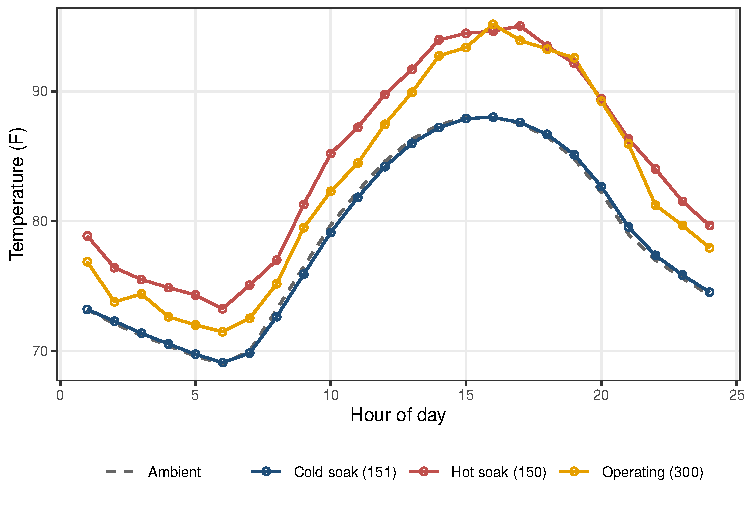
\includegraphics[width=0.75\linewidth]{figures/fig4_tank_temperature} 

}

\caption{Average tank temperature of passenger cars (tank temperature group 3) in the District of Columbia on a July weekday: movesr (lines) and MOVES execution tables (circles), with the ambient temperature. \label{fig:tank}}\label{fig:fig-tank}
\end{figure}

\subsection{A MOVES behaviour: vapor venting depends on the hours of the
run}\label{a-moves-behaviour-vapor-venting-depends-on-the-hours-of-the-run}

MOVES restricts the worker's \texttt{HourDay} table to the hours
selected in the RunSpec, and the vapor-venting script joins both the
initial and the current hour of each cold soak to that table. Cold soaks
that began outside the selected hours therefore do not vent, and the
multiday terms, which are anchored at hour 1, disappear when hour 1 is
not selected. In a run with a single hour no cold-soak venting is left
at all; only hot-soak and operating venting remain. movesr reproduces
this when it is given the same hours (argument \texttt{tvv\_hours}) and
otherwise computes venting over the 24 hours, which is what a full-day
MOVES run gives.

Figure \ref{fig:venting} shows the size of the effect for gasoline
passenger cars in the District of Columbia. With 24 hours, movesr agrees
with the MOVES 24-hour run within \(3.1 \times 10^{-5}\). Computed as
single-hour runs, venting between 08 and 15 h falls to between 36 and
98\% of the full-day value, depending on hour and model year (for model
year 2015 at 10 h, 0.0422 instead of 0.0831 g per vehicle and hour).
After the hour of peak tank temperature the two coincide, because
cold-soak venting stops when tanks start to cool. The DMV events run
used hours 16 and 17; its venting rates are 2.3\% lower than those of
the 24-hour run at 16 h for model year 2015, and they match the movesr
single-hour computation within \(1.3 \times 10^{-5}\). For inventories,
venting factors should come from full-day runs.

\begin{figure}[htbp]

{\centering 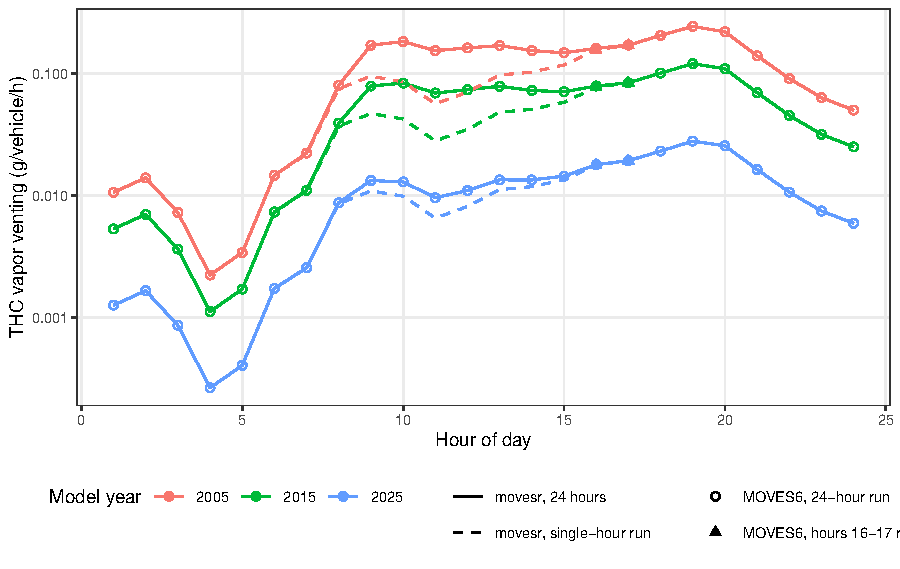
\includegraphics[width=0.85\linewidth]{figures/fig5_venting_hours} 

}

\caption{THC vapor venting of gasoline passenger cars in the District of Columbia, July weekday. Solid lines: movesr over 24 hours; dashed lines: movesr computing each hour as a single-hour run, as MOVES does; circles: MOVES6 24-hour run; triangles: MOVES6 run with hours 16 and 17. \label{fig:venting}}\label{fig:fig-venting}
\end{figure}

\subsection{Simplified evaporative
method}\label{simplified-evaporative-method-1}

The simplified method was tested on 20 MOVES default profiles not in the
library, with daily means from -14 to 25 C, for weekdays and weekends
(Figure \ref{fig:simple}). Daily totals of permeation and leaks differed
from the exact port by at most 0.44\%. Vapor venting differed by 3.8\%
on average. Excluding profiles farther than 5 F from the library, the
largest venting difference was 10\%. The method issued its warning for 2
test profiles (daily mean -14.3, 21.4 C), where the venting difference
reached 54\%. In a diagnostic run on two test profiles, made with an
earlier and smaller library, replacing the interpolated hot-soak shares
by the exact ones removed almost all of the venting error, while exact
tank temperatures or initial-hour fractions changed little. The hot-soak
share depends on how fast tanks cool towards the ambient temperature
over the whole day, which two daily statistics describe only roughly.

\begin{figure}[htbp]
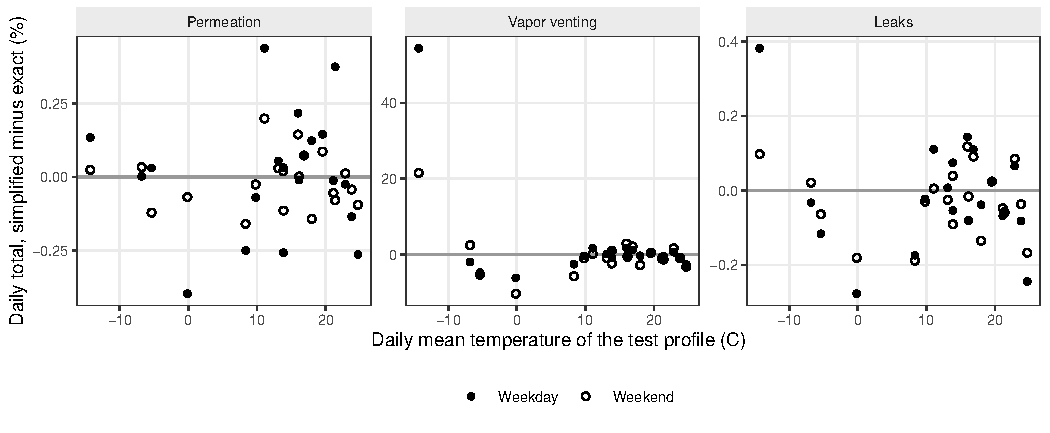
\includegraphics[width=1\linewidth]{figures/fig6_simplified} \caption{Daily totals of the simplified evaporative method relative to the exact port, for MOVES default temperature profiles not used to build the library. \label{fig:simple}}\label{fig:fig-simple}
\end{figure}

\subsection{From movesr to VEIN in the District of
Columbia}\label{from-movesr-to-vein-in-the-district-of-columbia}

Running NOx, CO, VOC and PM2.5 and brake PM2.5 rates for passenger cars,
passenger trucks and combination long-haul trucks in the District of
Columbia (July, 16 h) were exported with
\texttt{movesr\_export\_vein()}, read with
\texttt{vein::moves\_factors()} and evaluated with
\texttt{vein::ef\_moves()} at one speed inside each MOVES speed bin. All
720 values agreed with the MOVES DMV run within \(5.1 \times 10^{-6}\)
(Figure \ref{fig:vein}). For this, VEIN was extended to read brake, tire
and on-road evaporative rates, and its documentation of evaporative
units was corrected: MOVES writes all three evaporative processes as
grams per vehicle in the hour, including vapor venting in
\texttt{RatePerProfile}.

\begin{figure}[htbp]
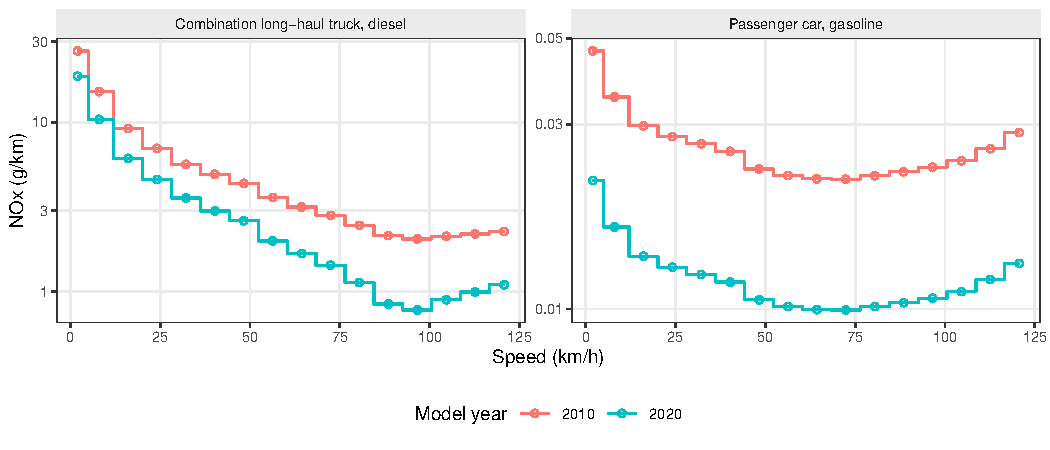
\includegraphics[width=1\linewidth]{figures/fig7_vein_dc} \caption{NOx emission factors in the District of Columbia (July, 16 h) evaluated by VEIN from movesr factors (steps) and the MOVES6 rates of the same bins (circles). \label{fig:vein}}\label{fig:fig-vein}
\end{figure}

\subsection{\texorpdfstring{Computing time
\label{sec:time}}{Computing time }}\label{computing-time}

\begin{table}

\caption{\label{tab:timing-table}Wall-clock time (minutes) and peak memory (GB) of the MOVES6 reference runs and of movesr computing the same rates on the same workstation. MOVES6: one run each, including start and shutdown of its MariaDB server; the Java column is the time reported by MOVES itself. movesr: three runs in fresh R processes, including R start-up and reading the database. Ratio: MOVES6 total over movesr median. Memory: largest resident set of a single process (GNU time), so the MOVES value is the larger of its Java program and its database server. \label{tab:time}}
\centering
\resizebox{\textwidth}{!}{\begin{tabular}[t]{>{\raggedright\arraybackslash}p{4.6cm}rrrrrrr}
\toprule
Workload & MOVES6 total & MOVES6 Java & movesr median & movesr range & Ratio & MOVES6 memory & movesr memory\\
\midrule
DMV running set: running, brake, tire (21 pollutants) and on-road evaporative (5 HC), 3 counties, 2 h & 57.9 & 55.4 & 6.3 & 6.2 to 6.3 & 9.2 & 0.8 & 2.4\\
DMV events set: start (21 pollutants) and parked evaporative (5 HC), 3 counties, 2 h & 9.9 & 9.3 & 2.7 & 2.6 to 2.7 & 3.7 & 0.7 & 0.8\\
DC evaporative, 24 h, exact tank model & 5.9 & 5.4 & 0.9 & 0.9 to 0.9 & 6.7 & 0.6 & 0.7\\
DC evaporative, 24 h, simplified tank model &  &  & 0.6 & 0.6 to 0.6 &  &  & 0.7\\
\bottomrule
\end{tabular}}
\end{table}

Table \ref{tab:time} compares the time needed to produce the same rates.
The measurements were made one after the other on a shared workstation
(Intel Xeon Gold 5215, 40 hardware threads, 85 GB of memory) while an
unrelated R process kept about one core busy and held 53 GB of memory,
so absolute times will differ on other machines. MOVES ran with one
worker, as in all reference runs. MOVES can distribute its work over
several workers, which we did not test; movesr runs in one thread. With
these settings movesr produced the same rates 3.7 to 9.2 times faster.
The largest gain was for the running set (9.2 times). We did not profile
MOVES, so we cannot say where its time goes; its log shows that the
running run was split into 672 bundles, each sent to the worker,
computed with its own SQL scripts and tables, and returned to the
master.

The gains have costs. movesr keeps whole tables in memory and needed 3.1
times more memory than the largest MOVES process for the running set.
The simplified evaporative method saves less time than one might expect:
38 s against 53 s for the DC 24-hour workload, because the tank
temperature simulation is only part of the work; starting R, reading the
database, computing activity and running the calculators take the rest.
Its advantage appears only when many temperature profiles are processed
in one session, where each exact simulation took 5 to 14 s in our tests
and each interpolation 0.2 s.

\section{Discussion}\label{discussion}

\subsection{\texorpdfstring{What makes the numbers equal
\label{sec:quirks}}{What makes the numbers equal }}\label{what-makes-the-numbers-equal}

Equality across MOVES, movesr and VEIN depends on a short list of
conditions. The MOVES version and default database must be the same,
because EPA updates rates and activity between releases. The inputs must
be the same, including details that are easy to overlook: the day type,
the hours selected (vapor venting), the 24-hour temperature profile (all
evaporative processes, even when only one hour is reported), and whether
ages with no population are expected to give zero or no rate. Several
MOVES steps are only defined by their code, and some of them differ from
what the documentation or the SQL suggests. The ones we found while
porting are:

\begin{itemize}
\tightlist
\item
  drive-cycle operating modes come from the Go generator, with zero
  acceleration after missing seconds;
\item
  \texttt{EmissionRateAdjustment} and temperature adjustments can have
  several model-year ranges for the same key;
\item
  energy is written in the unit of the RunSpec (joules here);
\item
  ages with \texttt{ageFraction\ =\ 0} give a zero rate in
  \texttt{RatePerDistance} and \texttt{RatePerStart}, and a NULL rate
  for on-road evaporative emissions;
\item
  evaporative rates are computed per regulatory class even when the
  output is not;
\item
  \texttt{stmyTVVEquations} stores the leak fraction already multiplied
  by the regulatory-class fraction, and the vented vapor is multiplied
  by that fraction again;
\item
  vapor venting depends on the hours selected in the run; single-hour
  runs lose all cold-soak venting (Figure \ref{fig:venting});
\item
  the E85 tank fuel used for vapor venting is not the same in every run.
  \texttt{FuelEffectsGenerator} replaces the properties of E85
  formulations with E10 values (cloning formulations per fuel-supply
  usage), and \texttt{TankFuelGenerator} reads the same table. In two of
  our runs (DMV events and DC 24 h) the venting rates match the E85
  formulation as supplied; in the other two that contain venting (DMV
  running, Washtenaw events) they match the E10-substituted formulation.
  We did not find what decides this; it is not simply whether exhaust
  processes are in the run, since the Washtenaw and DMV events runs have
  the same processes. The effect on E85 venting was 0.4\% in the DMV
  running run and up to 1.7\% in the Washtenaw run. movesr offers both
  (\texttt{e85\_tank\_properties\ =\ "raw"} or \texttt{"e10"}) and uses
  the first by default; users who need to match a particular MOVES run
  may have to try both.
\end{itemize}

A faithful port has to keep these behaviours, or document clearly where
it departs from them. movesr keeps them by default, with two exceptions
chosen for inventory use: venting is computed over 24 hours, and the
simplified evaporative method is available as an option.

\subsection{Is it good enough?}\label{is-it-good-enough}

movesr does not need to be identical to MOVES to the last bit to be
useful, and it is not. What matters for an inventory is whether a
difference could change a result. For exhaust, brake and tire rates the
differences are at the precision MOVES itself writes, so an inventory
built from either set of factors is the same to six significant digits.
For evaporative rates the largest difference, 0.087\%, occurs in a few
E85 venting rates; a difference of this size does not change an
inventory reported to two or three significant digits. The simplified
evaporative method is a different matter: errors of a few percent in
vapor venting, and much larger ones outside its library, are acceptable
for screening or for very large batches of locations but not when
MOVES-equivalent results are required. Because the exact tank model now
takes seconds per county, month and day type, the exact method is
affordable for most inventories, and we recommend it by default.

Two further limits should be stated plainly. First, movesr is not EPA
software. It reproduces MOVES for research and inventory work, but
regulatory analyses such as State Implementation Plans and
transportation conformity must use MOVES. Second, the code was written
by a language model (Section \ref{sec:ai}). Where movesr was compared
with MOVES, that origin does not matter, because the comparison is the
evidence. Where it was not compared (next section), errors are possible
that a human porter might or might not have made, and users should
compare with MOVES for configurations that differ substantially from the
reference runs.

\subsection{Limits of the
verification}\label{limits-of-the-verification}

The comparison covers what the reference runs contain: two calendar
months, one year (2025), weekday rates for the DMV counties and weekend
rates for Washtenaw, urban unrestricted roads for distance rates, and
low-altitude counties. Weekend evaporative rates were compared for one
county and three hours only, and needed the E85 setting discussed above.
Other years (movesr uses the default population of the requested year,
which approximates MOVES growth for non-base years), rural and
restricted-access roads, high-altitude counties, user-supplied fuels and
inspection programs, and off-network links with operating time were not
compared with MOVES. They use the same code paths, but they have not
been tested against the model. Extended idle, auxiliary power units,
crankcase processes, refueling and air toxics are not ported.

movesr reproduces MOVES, and MOVES describes the U.S. fleet. Outside the
United States, weather, fuel, barometric pressure and inspection
programs can be replaced, but the technology of each model year, the
fleet composition within source types and the trip patterns remain those
of MOVES.

\subsection{Use for the Washington DC
inventory}\label{use-for-the-washington-dc-inventory}

For the DC application the workflow is: generate running, start, brake,
tire and evaporative factors for each county of the DC-MD-VA region with
\texttt{movesr\_region\_rates()}, using MOVES default weather or local
observations for the 24 hours of each month and day type; export them
with \texttt{movesr\_export\_vein()}; and combine them in VEIN with
link-level traffic. Because every factor type has been checked against
MOVES for three of these counties, differences between the VEIN
inventory and a MOVES inventory of the same area should be attributable
to activity, not to emission factors.

\section{Conclusions}\label{conclusions}

movesr reproduces the MOVES6.0.0 emission rates of running and start
exhaust, brake and tire wear and evaporative processes, including their
chained pollutants, without Java, MariaDB or MOVES. All 4,302,126 rates
of five reference runs were reproduced, within the six-digit precision
of MOVES output for exhaust, brake and tire, and within
\(8.7 \times 10^{-4}\) for evaporative rates. The factors pass to VEIN
unchanged, and producing them took 3.7 to 9.2 times less time than MOVES
with one worker on the same machine. A simplified evaporative method
gives permeation and leak totals within 0.44\% and vapor venting within
a few percent on average, but with larger errors for climates outside
its library; the exact method remains the default. The scripts that
produced every number in this paper are part of the repository, so the
comparison can be repeated whenever MOVES or movesr changes.

\section{\texorpdfstring{Declaration of generative AI and AI-assisted
technologies in the research and writing process
\label{sec:ai}}{Declaration of generative AI and AI-assisted technologies in the research and writing process }}\label{declaration-of-generative-ai-and-ai-assisted-technologies-in-the-research-and-writing-process}

The movesr source code, the comparison scripts, the VEIN changes
described above and the first draft of this manuscript were written by
Claude Opus 5.5 (Anthropic, 2026), a large language model from
Anthropic, accessed through GitHub Copilot (model identifier
\texttt{claude-opus-5.5}) and run as a coding agent in OpenCode
(OpenCode, 2026) during working sessions on 28 and 29 October 2026. The
agent read the MOVES source code, wrote and ran R code, compiled and ran
MOVES on the author's workstation to produce the reference runs,
compared the outputs and corrected the code when comparisons failed. The
author set the objectives and constraints (no Java or MariaDB at run
time, data.table, a separate package connected to VEIN through factor
files, original and simplified evaporative methods) and decided the
questions the agent raised. The evidence that the code is correct is the
comparison with MOVES reported here, which any reader can repeat with
the published scripts. After using these tools the author reviewed and
edited the content as needed and takes full responsibility for the
content of the publication.

\section{Code and data availability}\label{code-and-data-availability}

movesr is available at \url{https://github.com/atmoschem/movesr} under
the GPL (\textgreater= 2) licence, like MOVES. The manuscript, scripts
and the compact comparison results used for tables and figures are in
its \texttt{paper} directory. The VEIN interface is available at
\url{https://github.com/atmoschem/vein}. The MOVES exports used as
reference can be regenerated with the RunSpecs and the script in
\texttt{data-raw/dmv}; the Washtenaw reference set is distributed with
VEIN. The manuscript was prepared with rticles (Allaire et al., 2024)
and the figures with ggplot2 (Wickham, 2016).

\section{CRediT authorship contribution
statement}\label{credit-authorship-contribution-statement}

\textbf{Sergio Ibarra-Espinosa:} Conceptualization, Methodology,
Software, Validation, Formal analysis, Investigation, Data curation,
Visualization, Writing - original draft, Writing - review and editing,
Project administration. The use of a language model for software and
drafting is described in Section \ref{sec:ai}.

\section{Declaration of competing
interest}\label{declaration-of-competing-interest}

The author declares that he has no known competing financial interests
or personal relationships that could have appeared to influence the work
reported in this paper.

\section{Funding}\label{funding}

This research did not receive any specific grant from funding agencies
in the public, commercial, or not-for-profit sectors.

\section*{References}\label{references}
\addcontentsline{toc}{section}{References}

\phantomsection\label{refs}
\begin{CSLReferences}{1}{0}
\bibitem[\citeproctext]{ref-rticles}
Allaire, J., Xie, Y., Dervieux, C., others, 2024. {rticles}: Article
formats for {R Markdown} {[}WWW Document{]}. URL
\url{https://CRAN.R-project.org/package=rticles} (accessed 10.29.2026).

\bibitem[\citeproctext]{ref-claude}
Anthropic, 2026. {Claude Opus 5.5} {[}WWW Document{]}. URL
\url{https://www.anthropic.com/claude} (accessed 10.29.2026).

\bibitem[\citeproctext]{ref-datatable}
Barrett, T., Dowle, M., Srinivasan, A., Gorecki, J., Chirico, M.,
Hocking, T., Schwendinger, B., Krylov, I., 2026. {data.table}: Extension
of `data.frame` {[}WWW Document{]}. URL
\url{https://CRAN.R-project.org/package=data.table} (accessed
10.29.2026).

\bibitem[\citeproctext]{ref-movesr}
Ibarra-Espinosa, S., 2026b. {movesr}: A standalone {R} port of the
{MOVES} on-road emission-rate engine {[}WWW Document{]}. URL
\url{https://github.com/atmoschem/movesr} (accessed 10.29.2026).

\bibitem[\citeproctext]{ref-veinrepo}
Ibarra-Espinosa, S., 2026a. {vein}: Vehicular emissions inventories
{[}WWW Document{]}. URL \url{https://github.com/atmoschem/vein}
(accessed 10.29.2026).

\bibitem[\citeproctext]{ref-vein2018}
Ibarra-Espinosa, S., Ynoue, R., O'Sullivan, S., Pebesma, E., Fátima
Andrade, M. de, Osses, M., 2018. {VEIN} v0.2.2: An {R} package for
bottom-up vehicular emissions inventories. Geoscientific Model
Development 11, 2209--2229.
\url{https://doi.org/10.5194/gmd-11-2209-2018}

\bibitem[\citeproctext]{ref-ieee754}
{IEEE} standard for floating-point arithmetic, 2019. {IEEE}.
\url{https://doi.org/10.1109/IEEESTD.2019.8766229}

\bibitem[\citeproctext]{ref-jimenez1999}
Jiménez-Palacios, J.L., 1999. Understanding and quantifying motor
vehicle emissions with vehicle specific power and {TILDAS} remote
sensing (PhD thesis). Massachusetts Institute of Technology.

\bibitem[\citeproctext]{ref-opencode}
OpenCode, 2026. {OpenCode}: An open source coding agent {[}WWW
Document{]}. URL \url{https://opencode.ai} (accessed 10.29.2026).

\bibitem[\citeproctext]{ref-R}
R Core Team, 2021. R: A language and environment for statistical
computing {[}WWW Document{]}. URL \url{https://www.R-project.org/}
(accessed 10.29.2026).

\bibitem[\citeproctext]{ref-duckdb2019}
Raasveldt, M., Mühleisen, H., 2019. {DuckDB}: An embeddable analytical
database, in: Proceedings of the 2019 International Conference on
Management of Data, SIGMOD '19. ACM, pp. 1981--1984.
\url{https://doi.org/10.1145/3299869.3320212}

\bibitem[\citeproctext]{ref-parquet}
The Apache Software Foundation, 2026. {Apache Parquet} {[}WWW
Document{]}. URL \url{https://parquet.apache.org} (accessed 10.29.2026).

\bibitem[\citeproctext]{ref-moves6code}
U.S. Environmental Protection Agency, 2026c. {MOVES6.0.0}: Motor vehicle
emission simulator, source code (tag {MOVES6.0.0}, commit
45805553e5afb575ae2d29daf89fe1bdbe4b8e56; default database
movesdb20260729) {[}WWW Document{]}. URL
\url{https://github.com/USEPA/EPA_MOVES_Model} (accessed 10.29.2026).

\bibitem[\citeproctext]{ref-movesweb}
U.S. Environmental Protection Agency, 2026a. {MOVES} and mobile source
emissions research {[}WWW Document{]}. URL
\url{https://www.epa.gov/moves} (accessed 10.29.2026).

\bibitem[\citeproctext]{ref-moves6guidance}
U.S. Environmental Protection Agency, 2026b.
\href{https://www.epa.gov/moves/latest-version-motor-vehicle-emission-simulator-moves}{{MOVES6}
technical guidance: Using {MOVES} to prepare emission inventories for
state implementation plans and transportation conformity} (No.
EPA-403-B-26-002). {Office of Transportation and Air Quality}.

\bibitem[\citeproctext]{ref-greenbook}
U.S. Environmental Protection Agency, 2026d. Nonattainment areas for
criteria pollutants ({Green Book}) {[}WWW Document{]}. URL
\url{https://www.epa.gov/green-book} (accessed 10.29.2026).

\bibitem[\citeproctext]{ref-ggplot2}
Wickham, H., 2016. \href{https://ggplot2.tidyverse.org}{ggplot2: Elegant
graphics for data analysis}. Springer-Verlag New York.

\end{CSLReferences}


\end{document}
